\chapter{Forensic audit and its computer support}


\komentar{na zacatek shrnout co vsechno obsahuje tato kapitola. asi tak takhle:}


This chapter strives to define and explain the meaning of the term "forensic audit" as well as other therms related to this field. We demonstrate typical roles and outline the process. 

\section{Definition of Forensic audit}
\komentar{co je to forenzni audit}
\sediva{ \blindtext}

\komentar{v hrubych rysech jak to probiha (to co uz mam sem patri), na zaklade toho, co jsem zjistila FA funguje takto:...\\}
\sediva{ \blindtext}


\begin{figure}[h]
	\begin{center} 
	\missingfigure{Obrazek demonstrujici forenzni audit.}
	%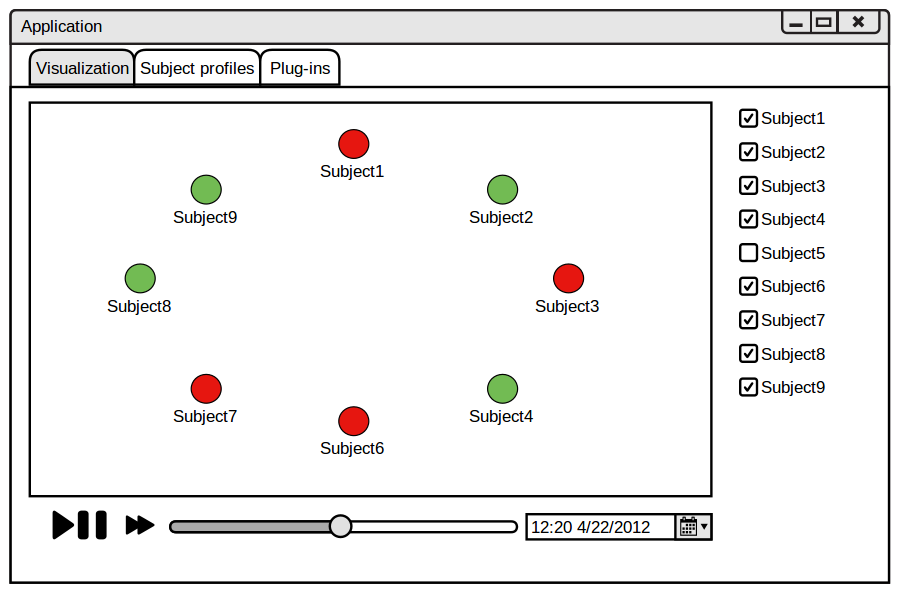
\includegraphics[width=1.0\textwidth]{img/GUI/visualization.png}
	\end{center}
	\caption{\komentar{popis obrazku}}
\end{figure}




\komentar{
\subsection*{use case diagram}
 komentar k diagramu
}


\sediva{ \blindtext}

\begin{figure}[h]
	\begin{center} 
	\missingfigure{Velky obrazek vsech zainteresovanych stran - f.auditor, datovy analytik pro FA, zakaznik (zadavatel, materska spolecnost)}
	%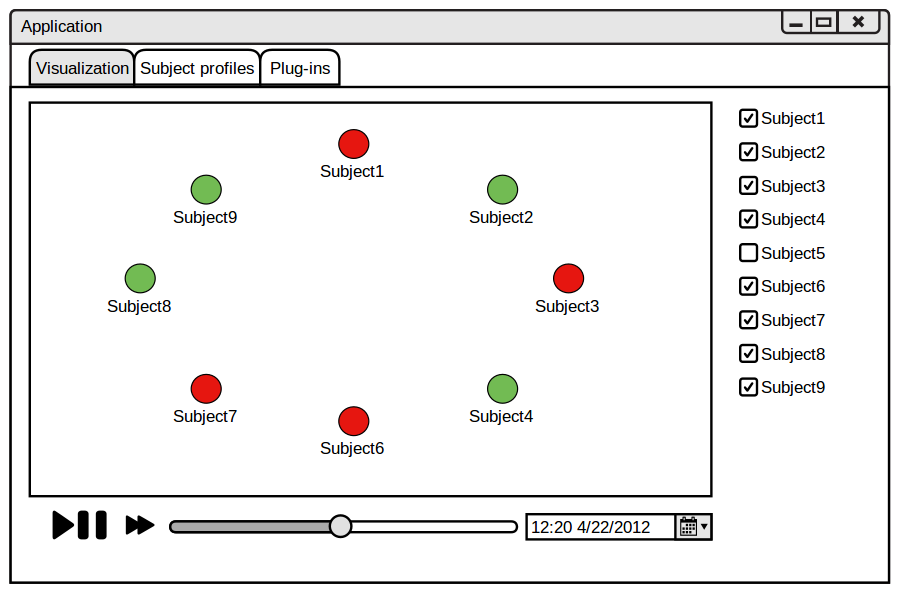
\includegraphics[width=1.0\textwidth]{img/GUI/visualization.png}
	\end{center}
	\caption{\komentar{popis obrazku}}
\end{figure}

